\subsection{Tag probability cross validation}
\label{sec:xval}

To test the bias of the background estimation a method of cross validation is utilized. For a given sample, $N_{\textrm{div}}$ non-overlapping  sub-samples are partitioned. 
For each sub-sample, a corresponding set of jet probabilities are computed as described in the previous section. 
For each set of jet probabilities, an $N_{\textrm{tags}}^{\textrm{pred}}$  prediction is made for the $N_{\textrm{div}}-1$ remaining samples (which have no overlapping events). We will
refer to the sample use for the prediction as the measurement sample. The result is $N_{\textrm{div}}(N_{\textrm{div}}-1)$ pairs of probabilities and measurement samples. 
From each pair, in each bin of $N_{\textrm{tags}}$, we  generate a distribution of pulls $(N_{\textrm{obs}} - N_{\textrm{pred}}) / \sqrt{N_{\textrm{pred}}}$ for each $N_{\textrm{tags}}$ bin. All events must pass the event selection. Due to limited statistics in the 2 tag bin for the baseline tag, the loose tag definition (Table \ref{tab:loose_tag_def}) is used to generate pull distributions in the 2 tag bin. 

\begin{figure}
\begin{center}
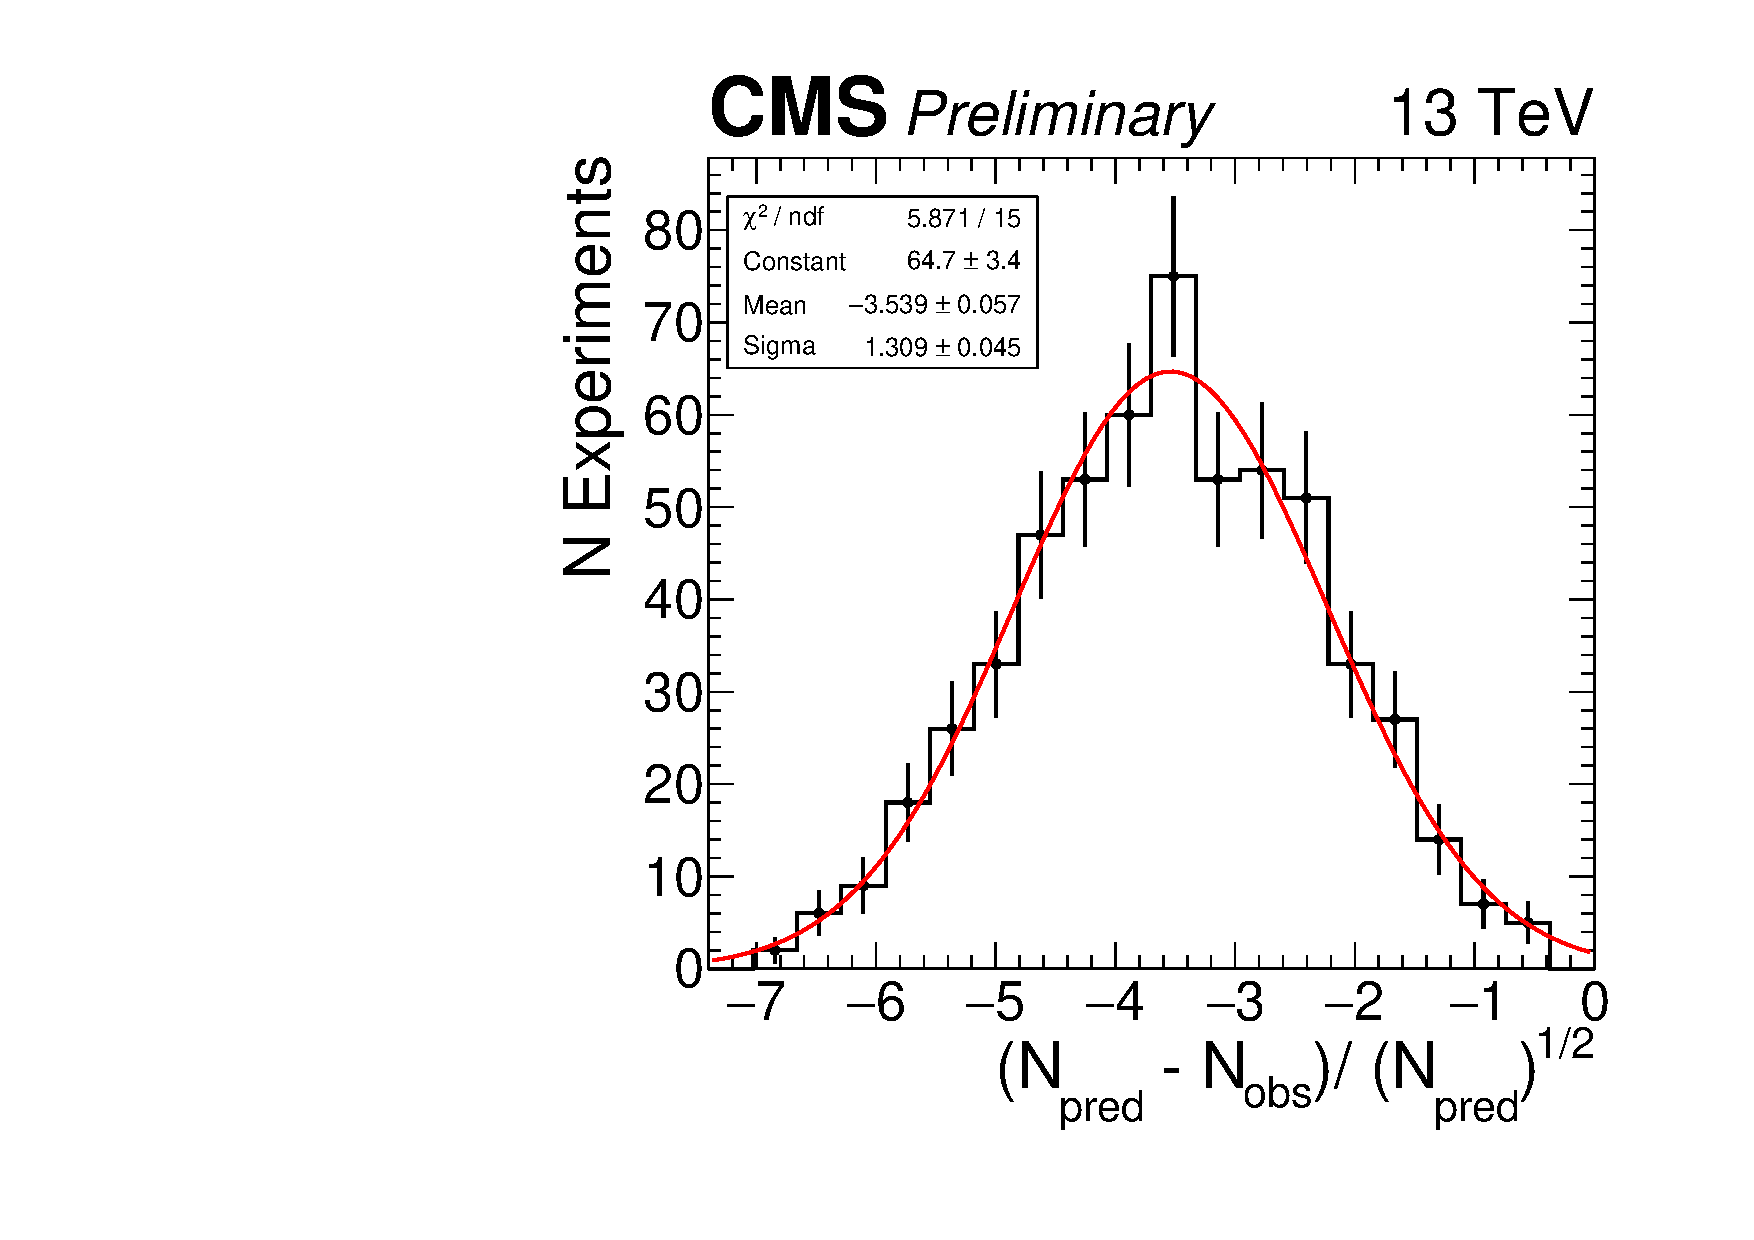
\includegraphics[width=.45\textwidth]{figures/an/ANALYSIS/pulls/data_loose_uncorrected_1tag.pdf}
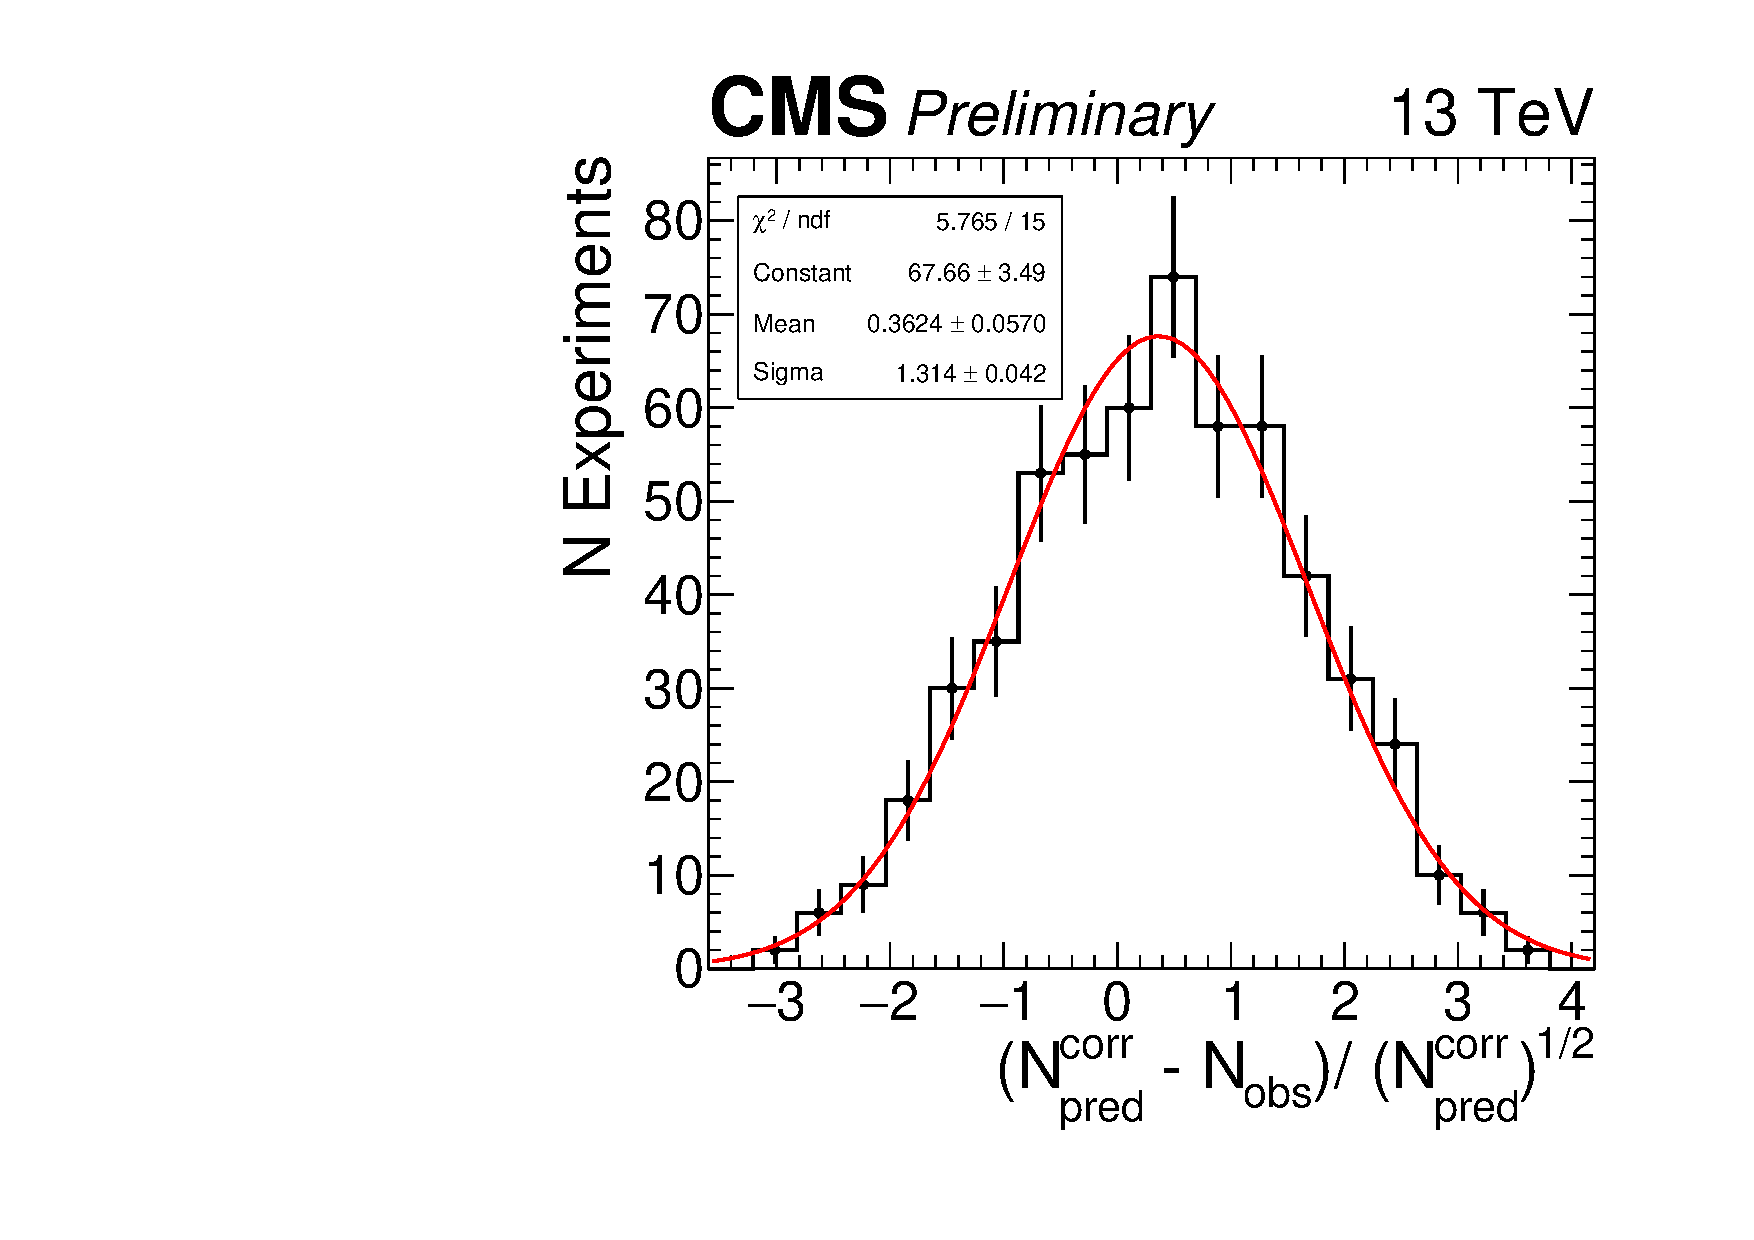
\includegraphics[width=.45\textwidth]{figures/an/ANALYSIS/pulls/data_loose_corrected_1tag.pdf}
\caption{(left) Cross validation of the predicted of the number of loose tags in data collected by the displaced jet triggers. Pulls for the 1 tag bin with the loose tag. (right) Pulls for the 1 tag bin with the loose tag with the SR correction .   \label{fig:djetpd_1tag_xval}}
\end{center}
\end{figure}

\begin{figure}
\begin{center}
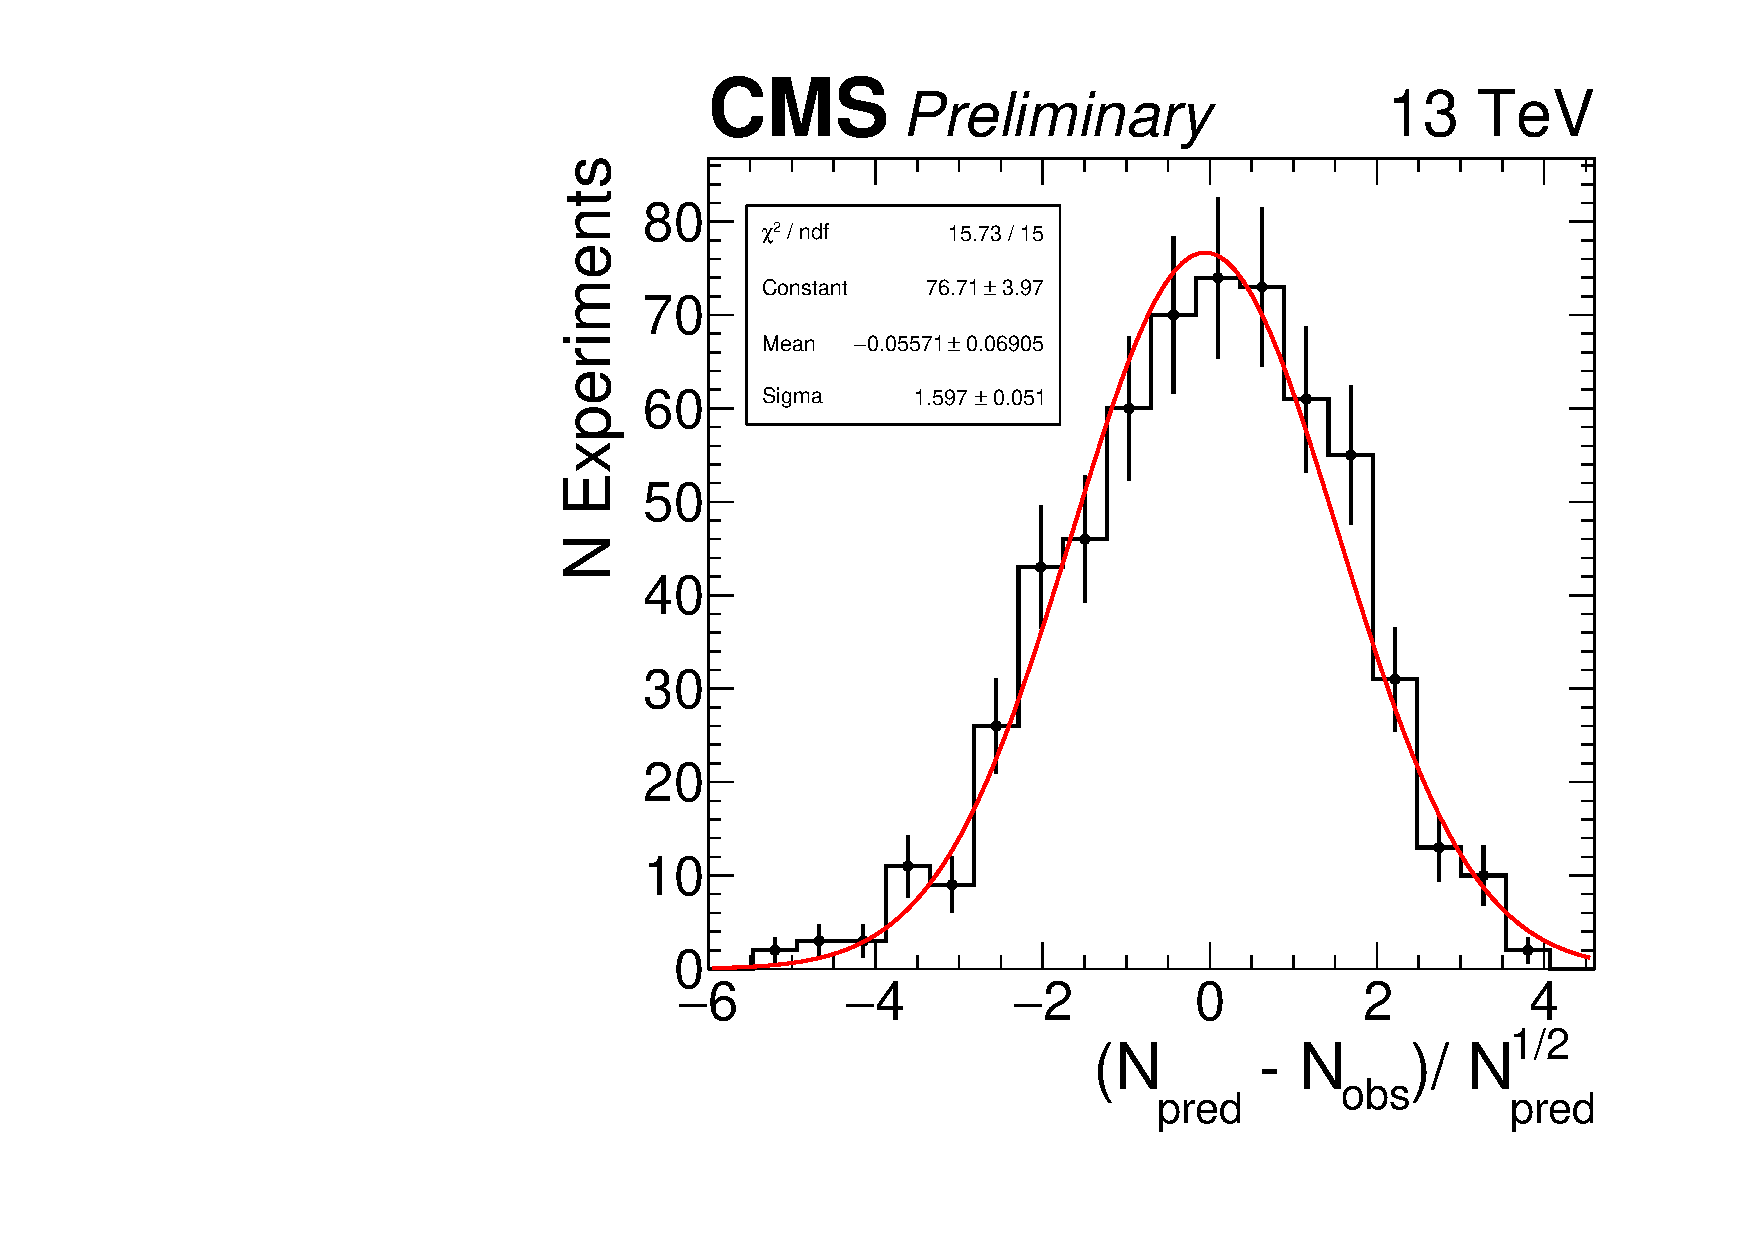
\includegraphics[width=.45\textwidth]{figures/an/ANALYSIS/pulls/baseline_xval_ndiv25_baseline_1tag.pdf}
\caption{Cross validation of the predicted of the number of tags in data passing the displaced jet triggers. Pulls for the 1 tag bin with the baseline tag after the application of the signal removal correction $2r_{12}=0.2\%$ \label{fig:djetpd_1tag_xval_baseline}}
\end{center}
\end{figure}

\begin{figure}
\begin{center}
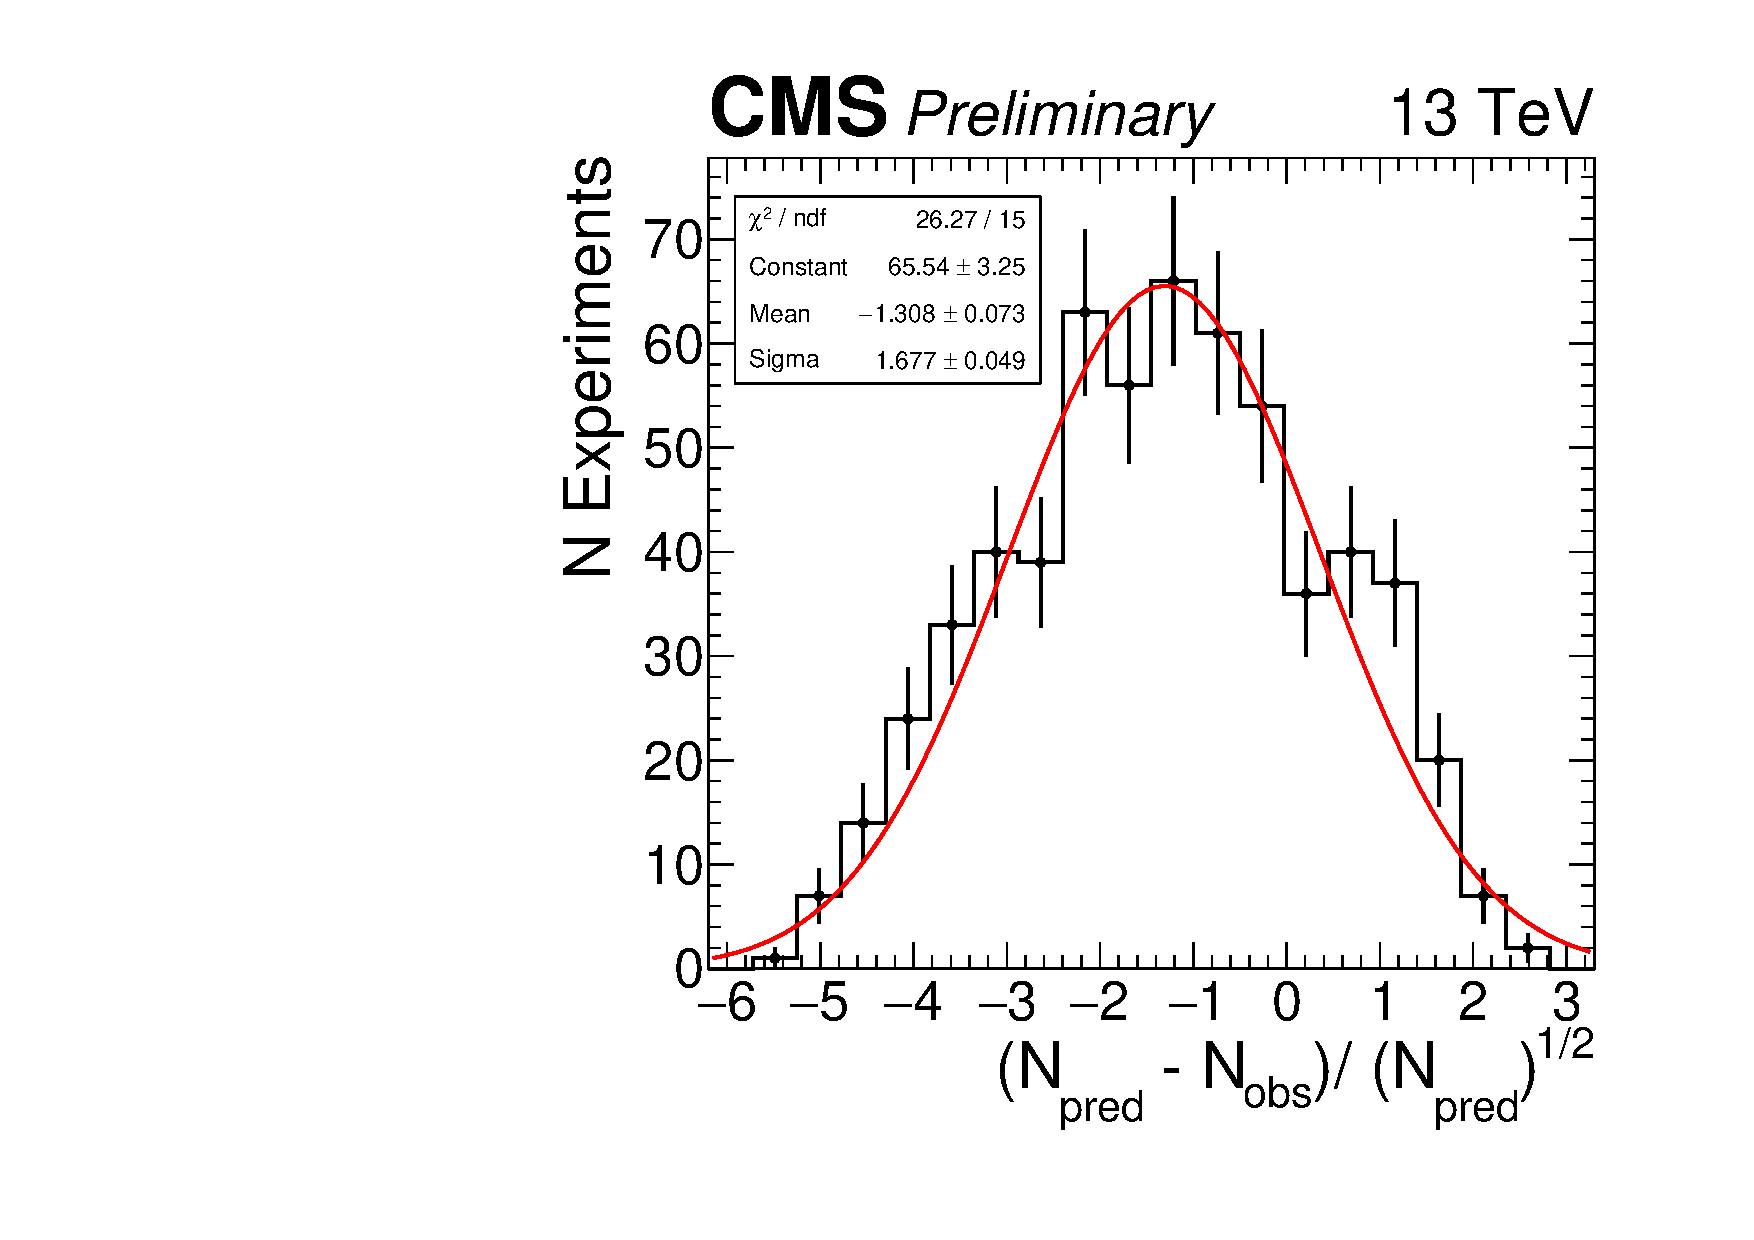
\includegraphics[width=.45\textwidth]{figures/an/ANALYSIS/pulls/qcd_loose_uncorrected_1tag.pdf}
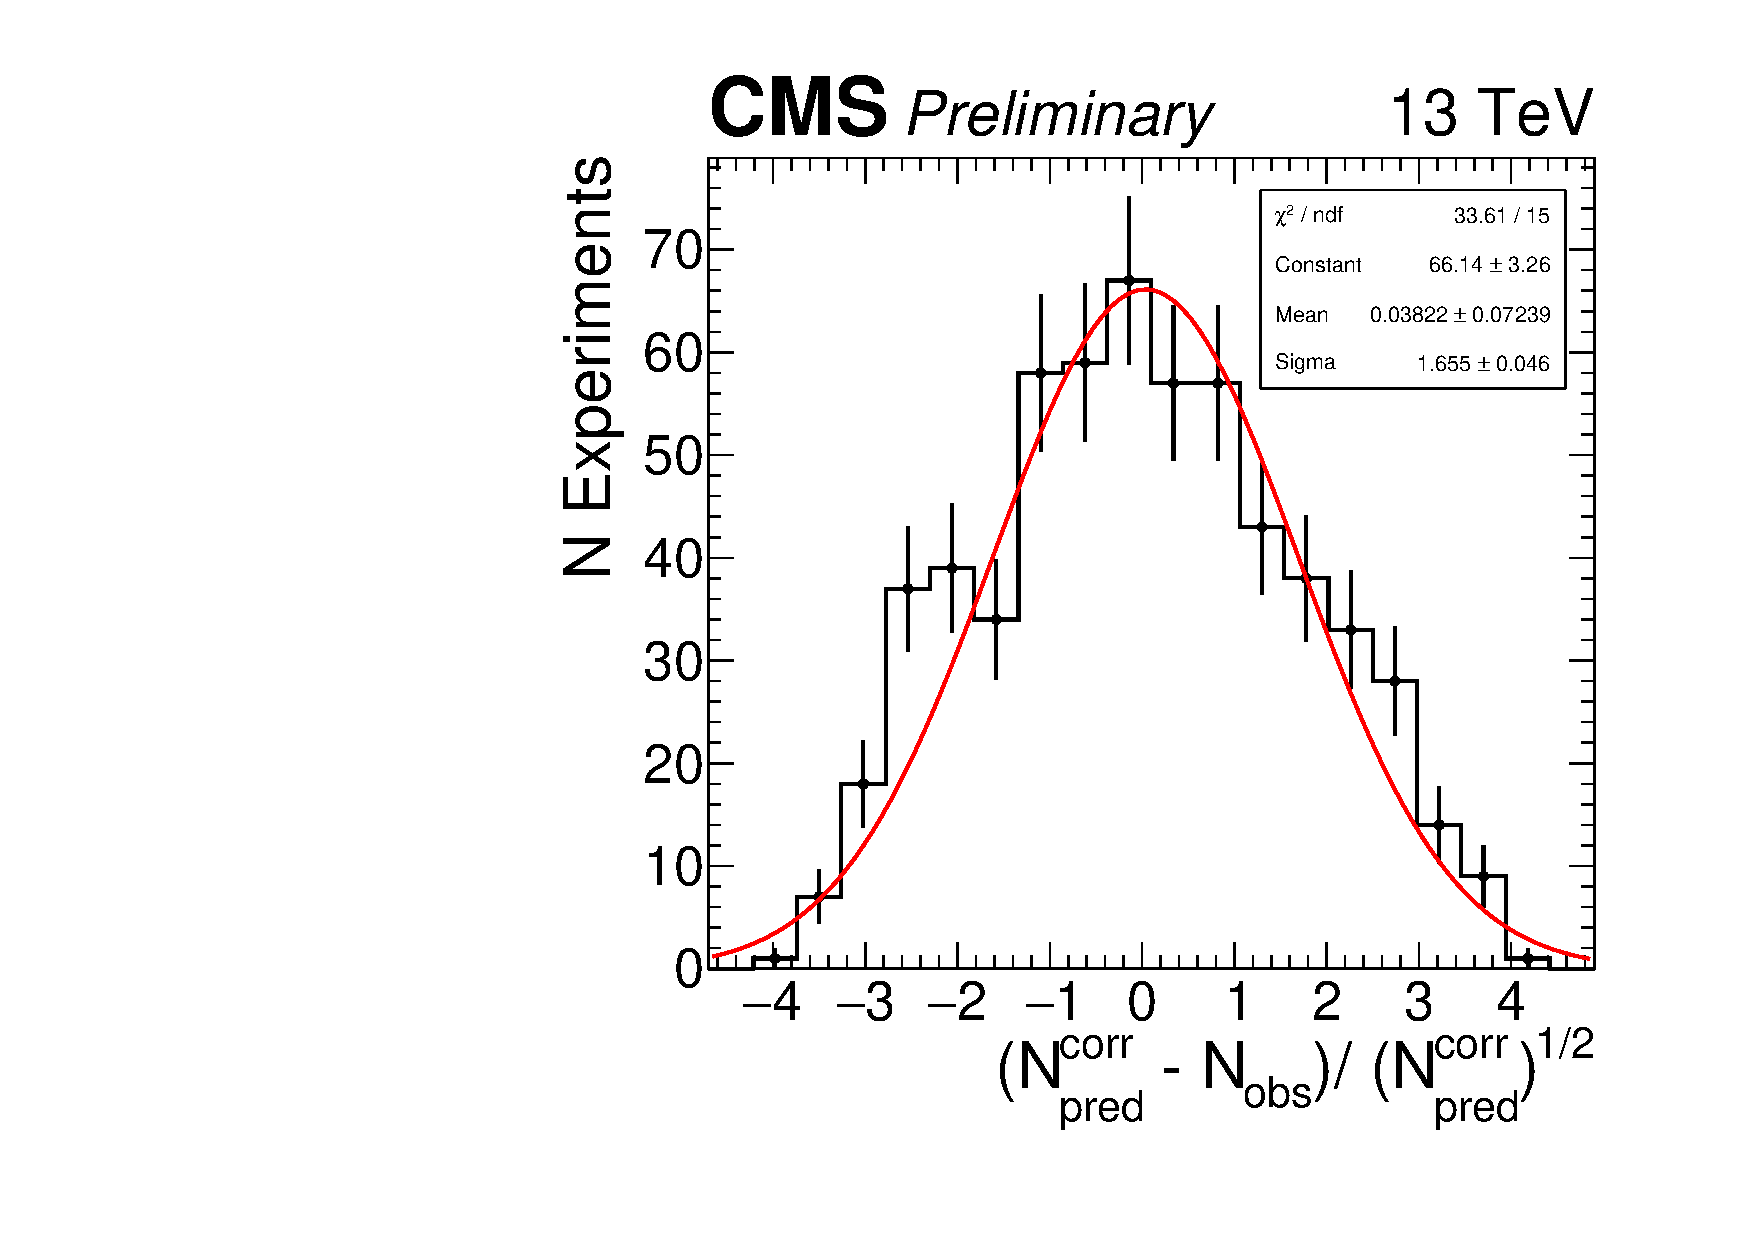
\includegraphics[width=.45\textwidth]{figures/an/ANALYSIS/pulls/qcd_loose_corrected_1tag.pdf}
\caption{(left) Cross validation of the predicted of the number of loose tags in QCD events passing the displaced jet triggers. Pulls for the 1 tag bin with the loose tag. (right) The signal region removal corrected pulls. \label{fig:qcd_1tag_xval}}
\end{center}
\end{figure}

\begin{figure}
\begin{center}
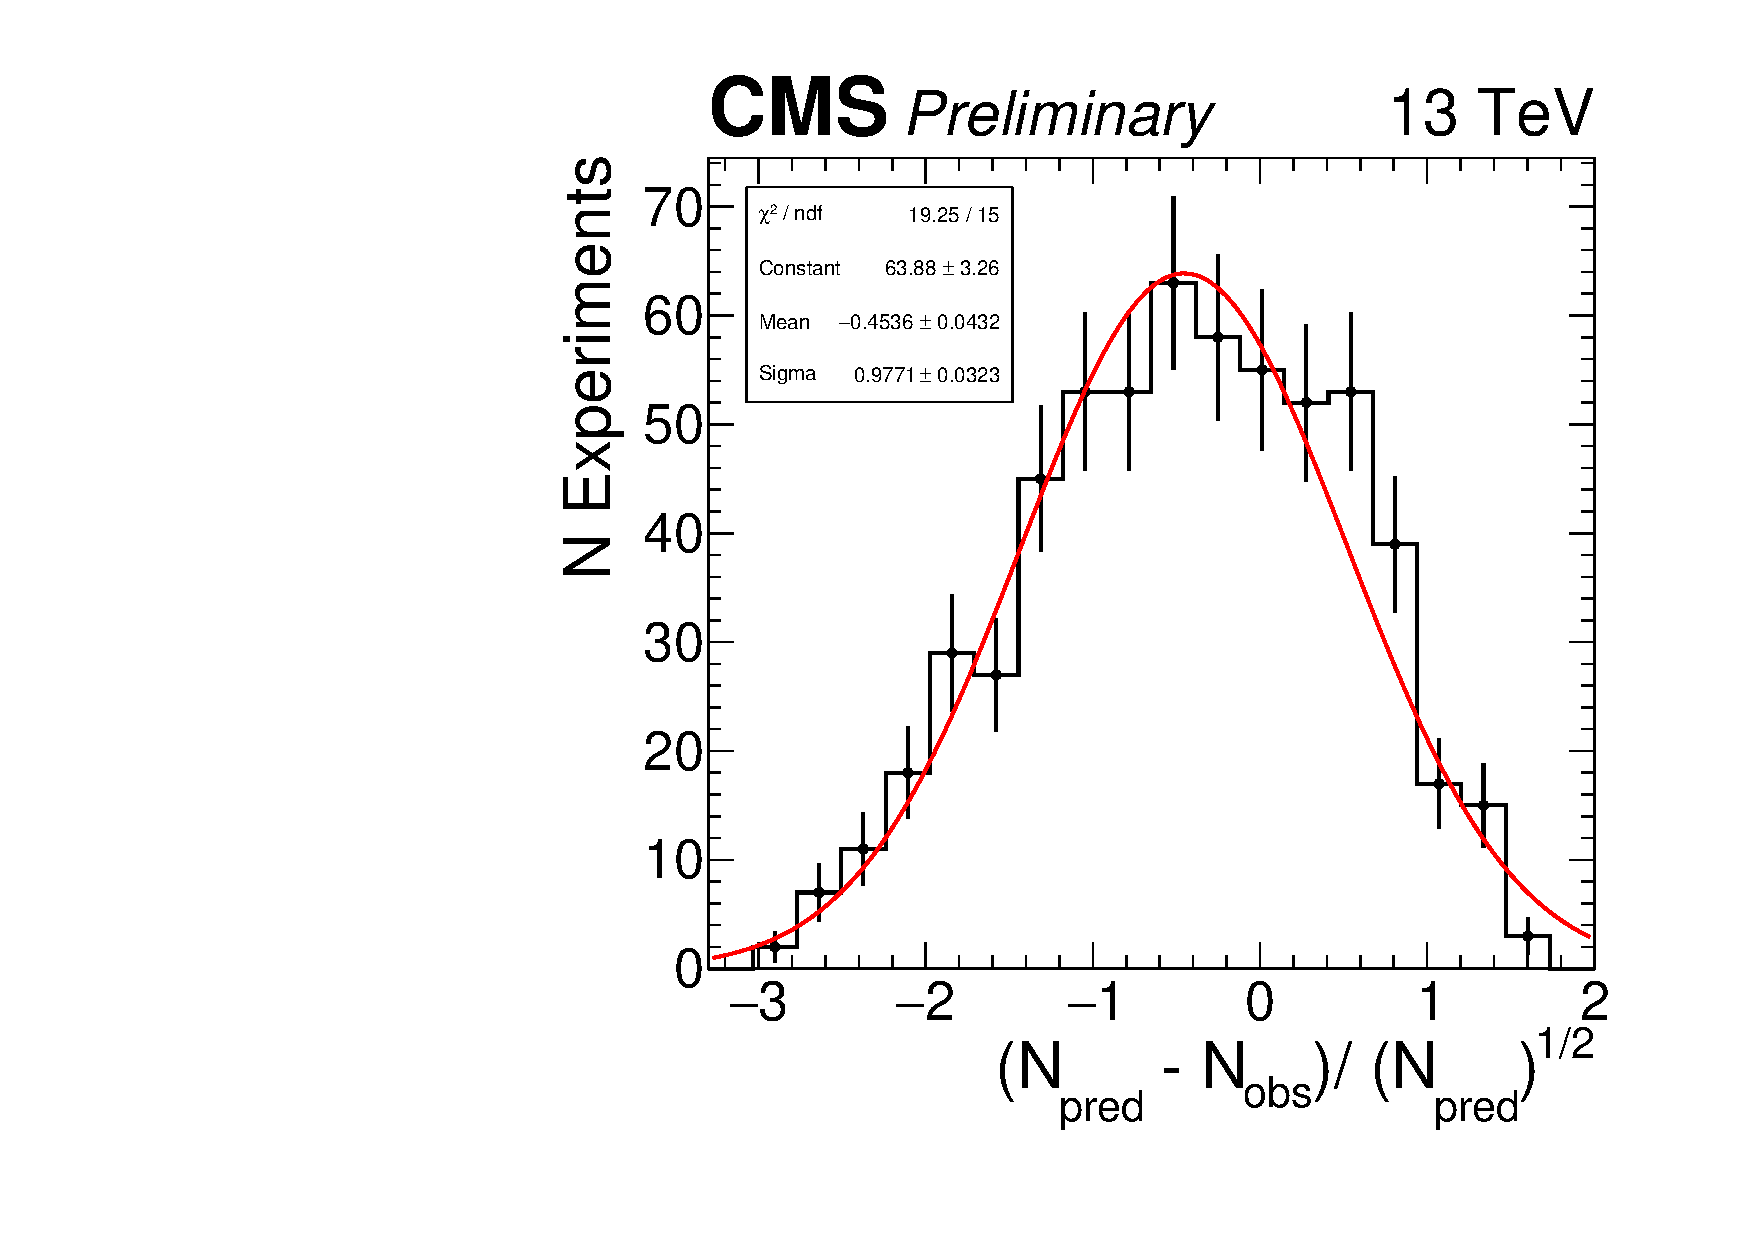
\includegraphics[width=.45\textwidth]{figures/an/ANALYSIS/pulls/qcd_loose_uncorrected_2tag.pdf}
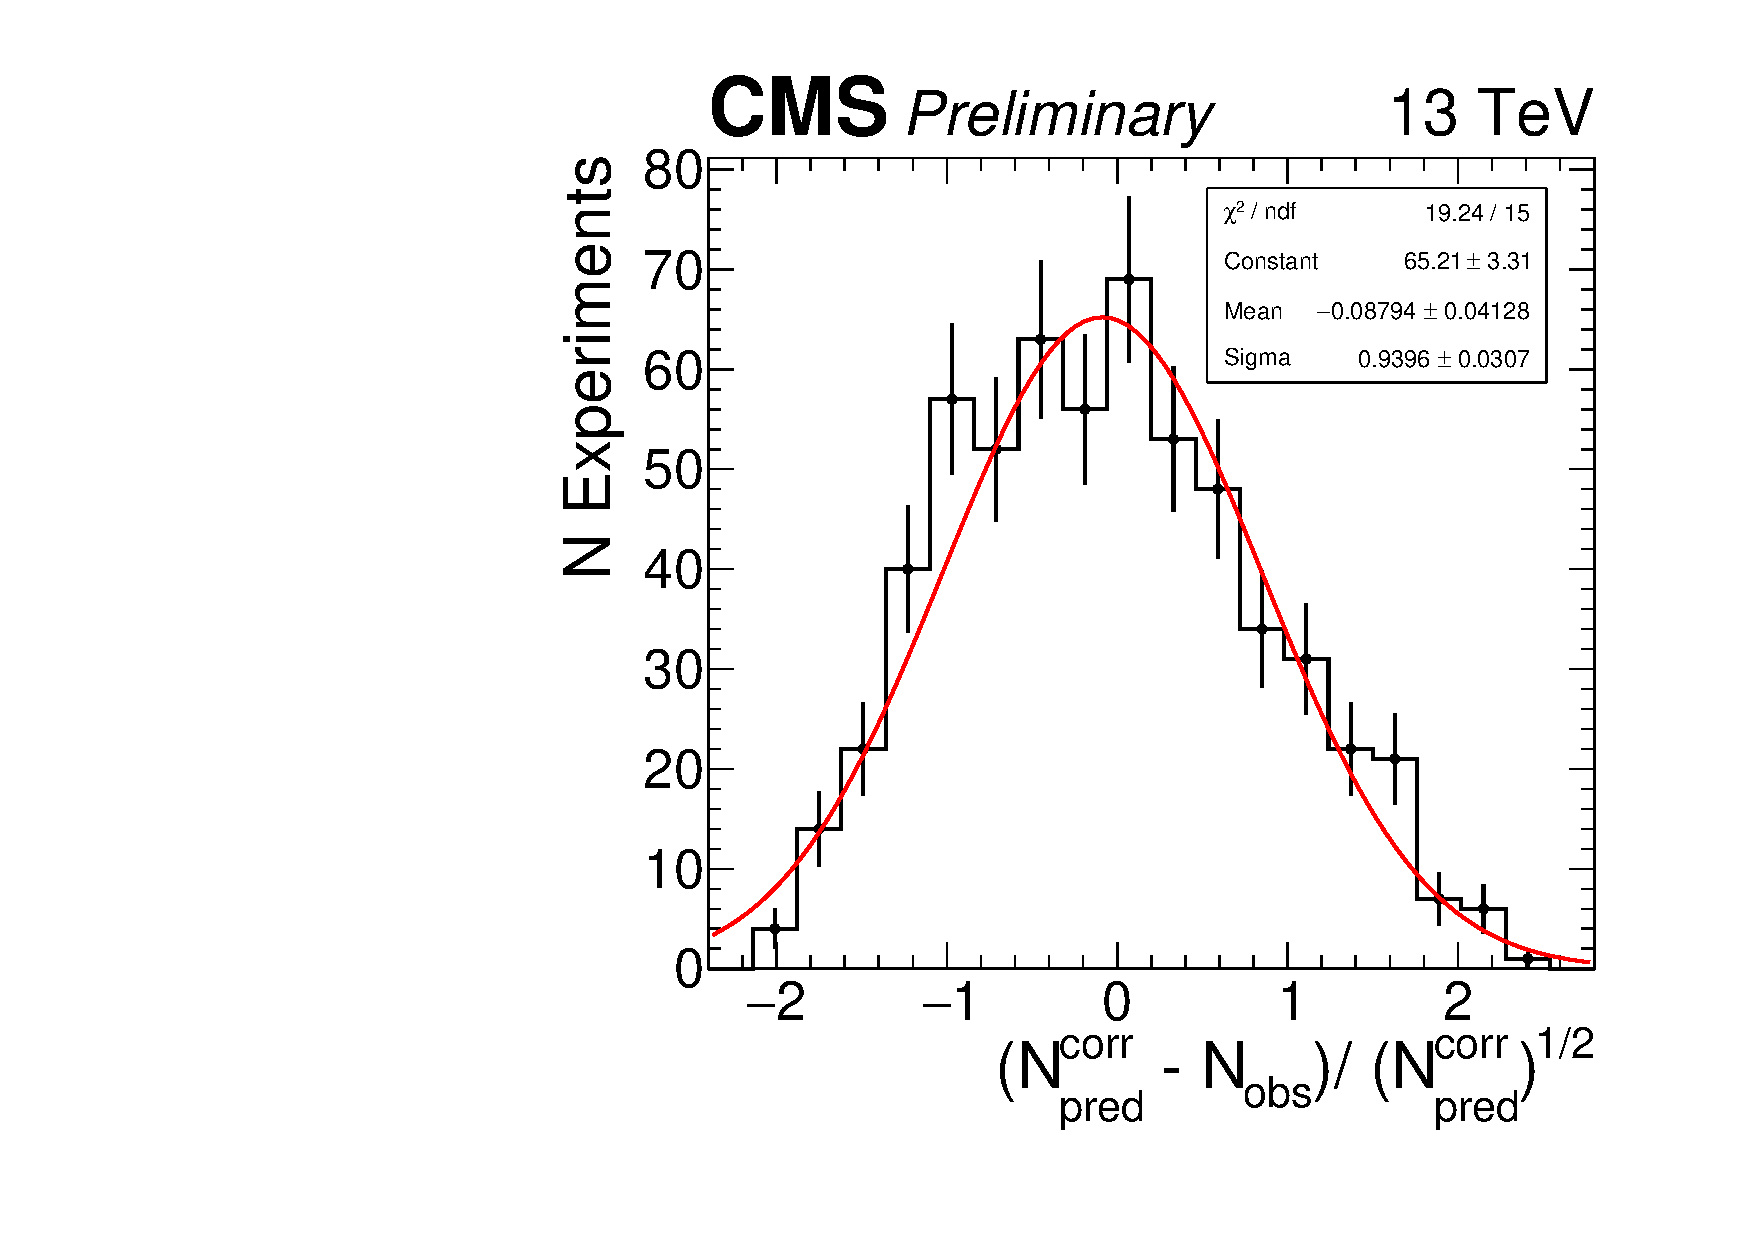
\includegraphics[width=.45\textwidth]{figures/an/ANALYSIS/pulls/qcd_loose_corrected_2tag.pdf}
\caption{(left) Cross validation of the predicted of the number of loose tag in QCD events passing the displaced jet triggers. Pulls for the 2 tag bin with the loose tag uncorrected. (right) The same prediction corrected for the SR removal  \label{fig:qcd_2tag_xval}}
\end{center}
\end{figure}


\begin{figure}
\begin{center}
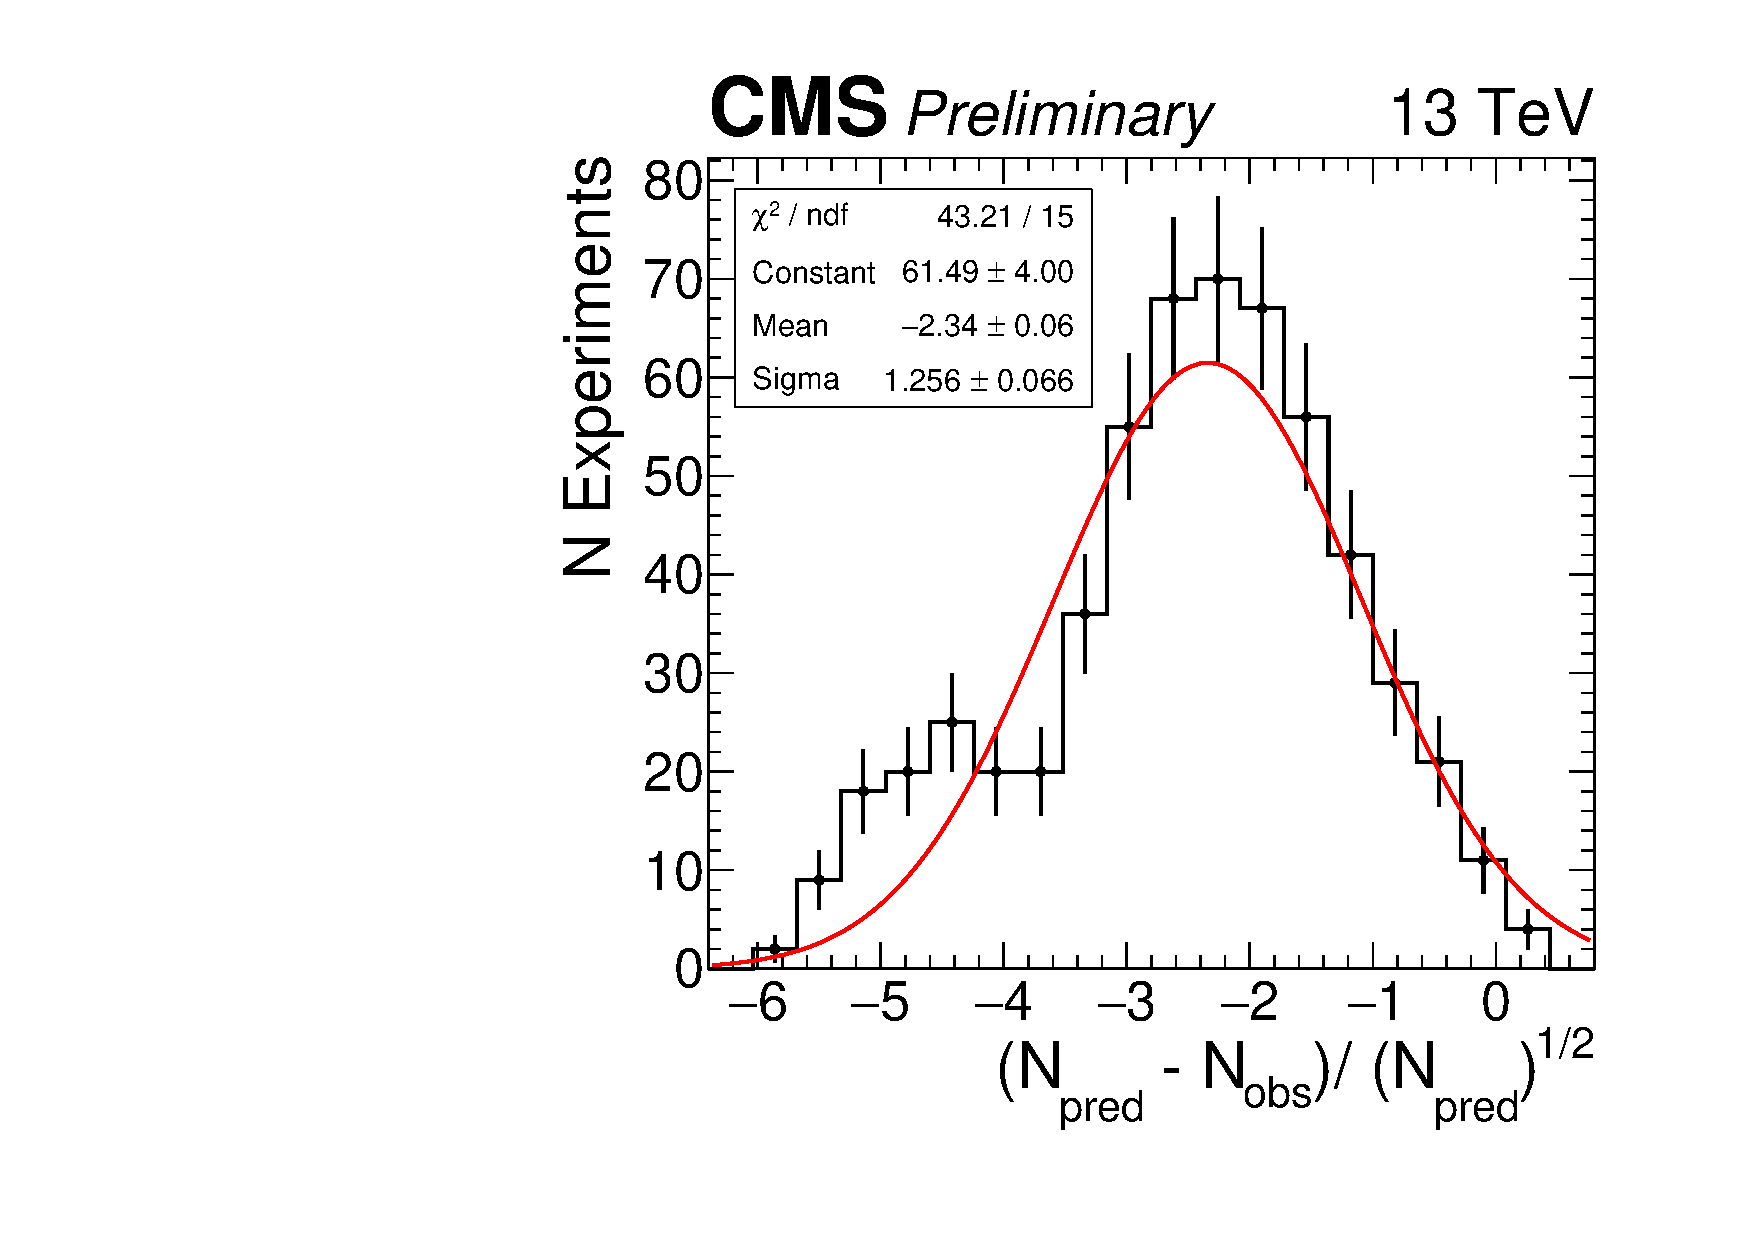
\includegraphics[width=.31\textwidth]{figures/an/ANALYSIS/pulls/data_loose_uncorrected_2tag.pdf}
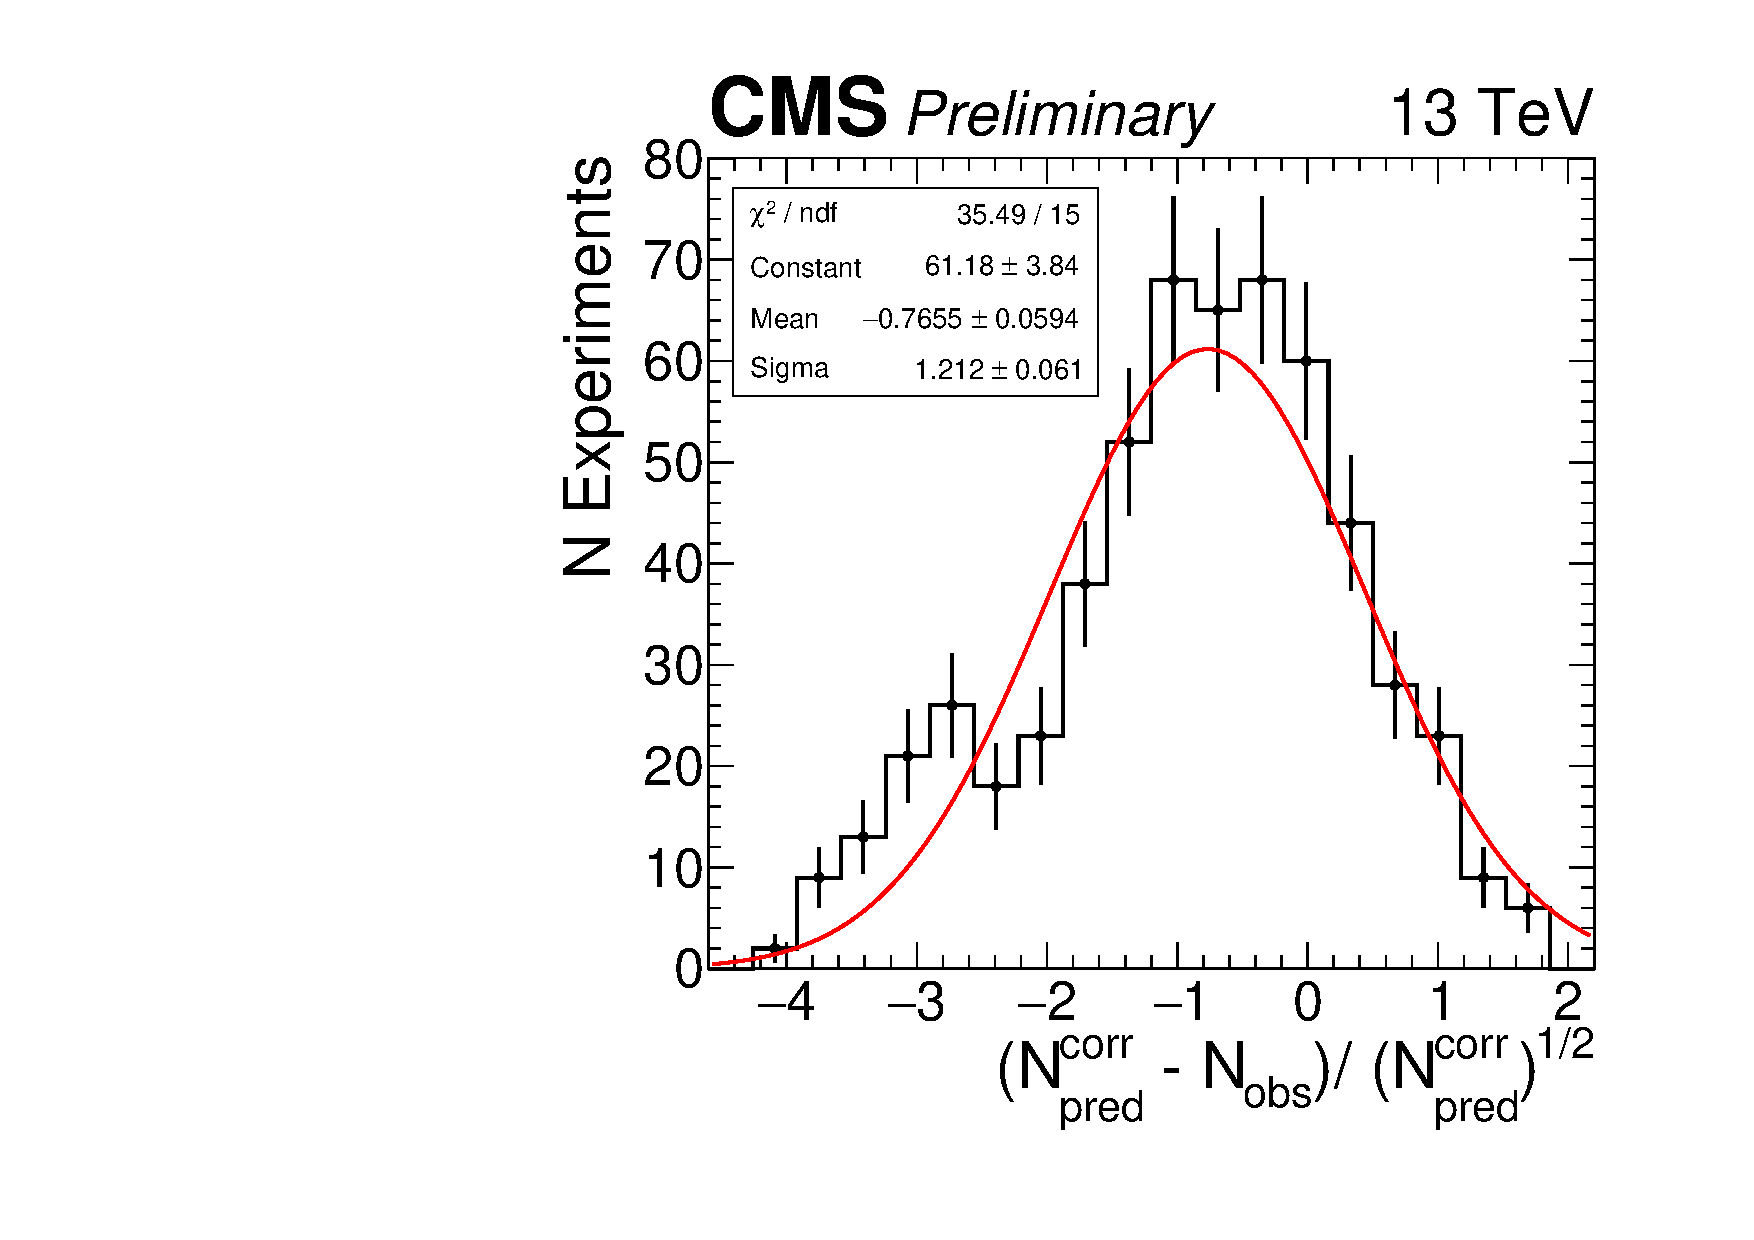
\includegraphics[width=.31\textwidth]{figures/an/ANALYSIS/pulls/data_loose_corrected_2tag.pdf}
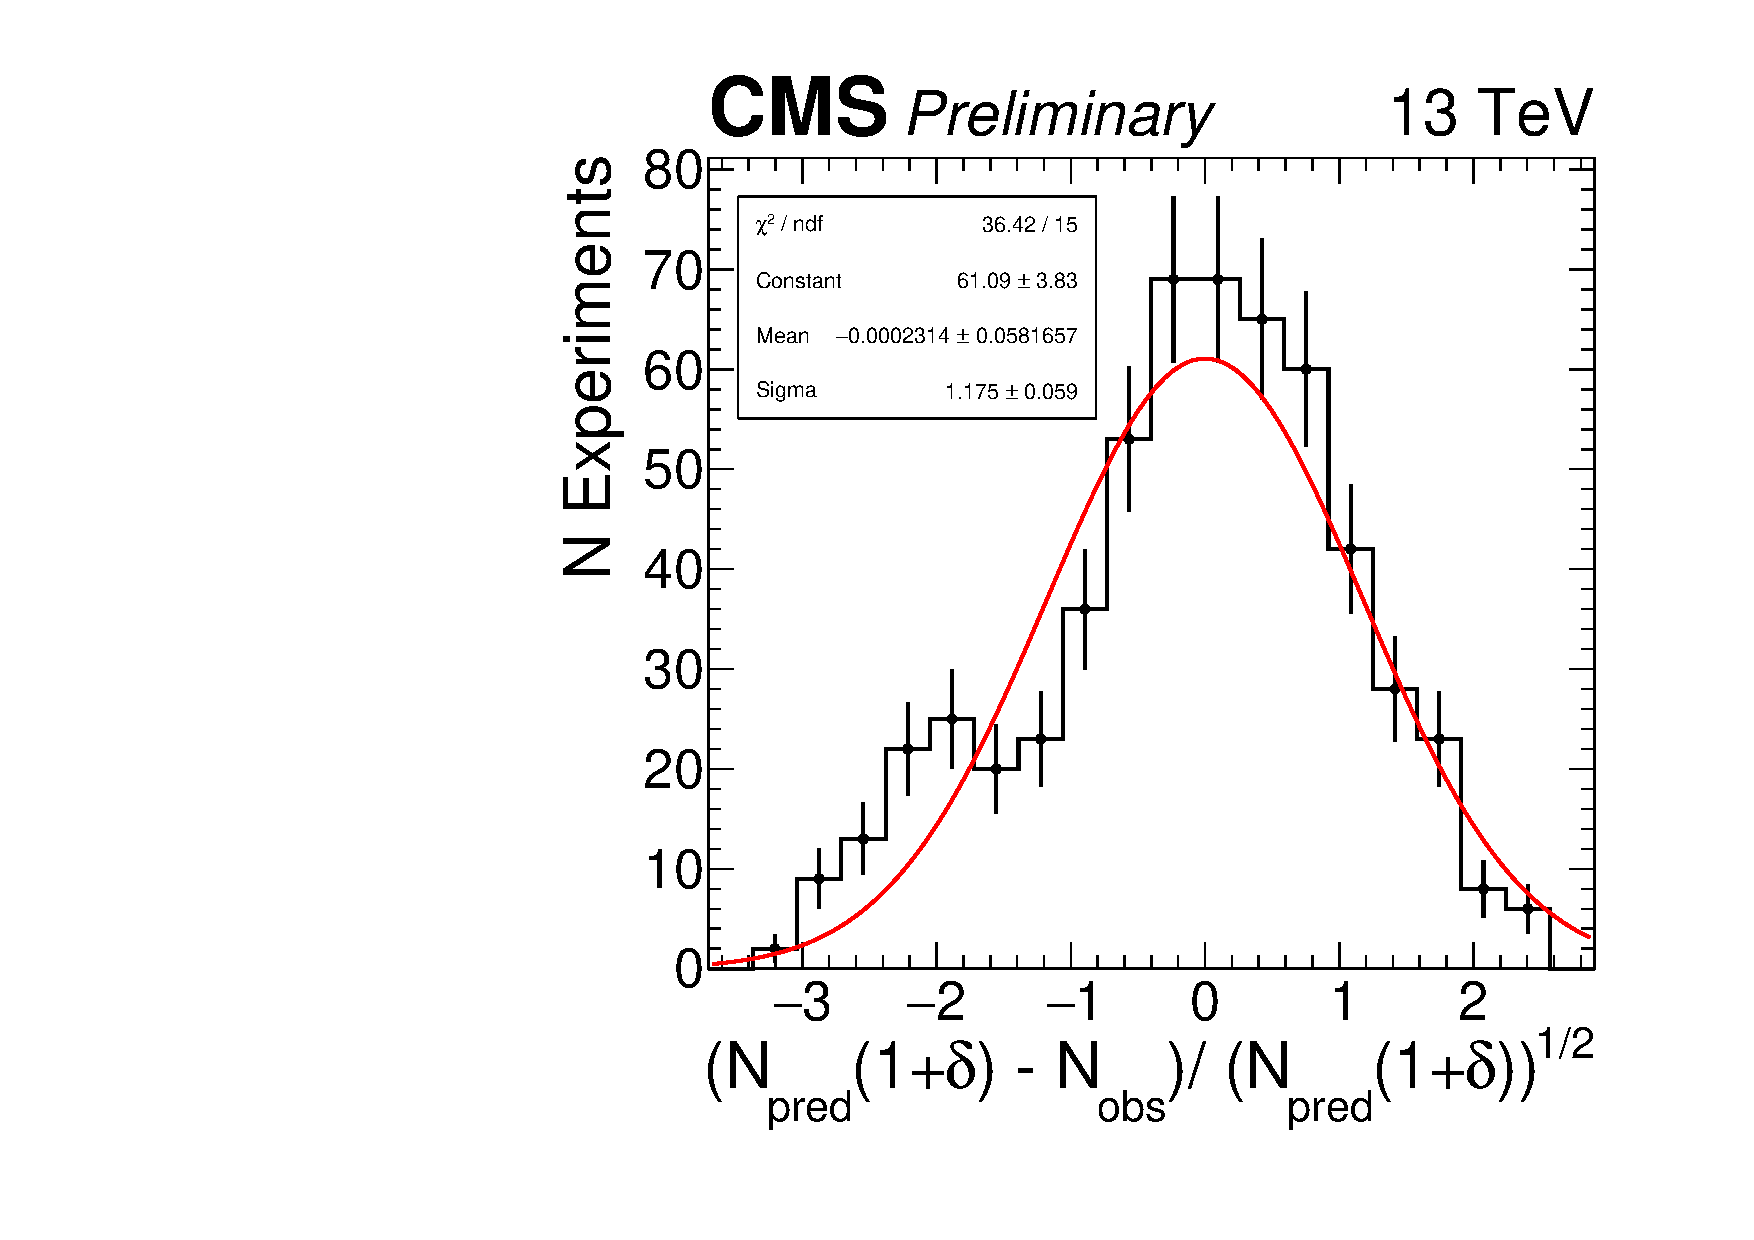
\includegraphics[width=.31\textwidth]{figures/an/ANALYSIS/pulls/data_loose_corrected_delta0p075_2tag.pdf}
\caption{(left) Cross validation of the predicted of the number of baseline tags in data collected by the displaced jet triggers. Pulls for the 2 tag bin with the loose tag. (right) Pulls with the signal region removal correction applied (middle). The same signal region removal correction shifted by $\delta=7.5\%$. 
\label{fig:djetpd_2tag_xval}}
\end{center}
\end{figure}

We summarize the cross validation studies in the following figures:
\begin{itemize}
\item Figure \ref{fig:djetpd_1tag_xval}: SR corrected and uncorrected 1 tag bin pulls for the loose tag definition in data collected by Displaced Jet Triggers. 
\item Figure \ref{fig:qcd_1tag_xval}: 1 tag bin pulls for the loose tag definition in QCD events passing the Displaced Jet Triggers. 
\item Figure \ref{fig:qcd_2tag_xval}: 2 tag bin pulls for the loose tag definition in QCD events passing by Displaced Jet Triggers. 
\item Figure \ref{fig:djetpd_2tag_xval}: SR corrected, uncorrected, and SR corrected+$\delta$ 2 tag bin pulls for the loose tag definition in data collected by Displaced Jet Triggers.
\end{itemize}

In data and QCD, the SR correction provides a significant improvement on the pull distributions with respect to the ideal parameters $\mu=0$ and $\sigma=1.0$. For the 1 tag prediction in data with the loose tag the central value changes from $\mu=3.5$ (uncorrected) to $\mu=0.36$ (corrected). For the signal region (2+ tags), the loose tag in data is within 7.5\% of ideal $\mu$ and the QCD estimate is within error of $\mu=0$ but has $\sigma=1.6>1.0$. 

%% The 1 tag pulls for both the baseline and loose tag definitions have a mean constient with 0. The level of consistency is at 1 $\sigma_{mu}$ and 2.1 $\sigma_\mu$ for the baseline and loose tag definitions respectively. The purely poission 
%% error predicts  pulls with $\sigma_{gaus}=1$. For the baseline and loose tag definitions we have $\sigma_{gaus} = 1.33$ and $1.21$ respectively.
%% The fact these are greater than 1 is due to inaccuracies in the prediction method as well as the statistical uncertainty in the fake rate measurement. 
